\documentclass[11pt]{article}

% ============================================================
% PACKAGES
% ============================================================

% Custom style: automatic header, footer and watermark
\usepackage{NAstyle}

\usepackage{geometry}
\usepackage{enumitem}
\usepackage{fontspec}
\usepackage{titlesec}
\usepackage{tabularx}
\usepackage{multicol}
\hypersetup{hidelinks}
\usepackage{url}
\urlstyle{tt}
% ============================================================
% PAGE LAYOUT
% ============================================================

\geometry{
    a4paper,
    left=1.2cm,
    right=1.2cm,
    top=1.5cm,
    bottom=1.8cm,
    nohead
}

\setlength{\parindent}{0pt}
\pagenumbering{gobble}

\setlist[itemize]{
    topsep=0.2em,
    itemsep=0.15em,
    leftmargin=*
}

\setlist[enumerate]{
    topsep=0em,
    leftmargin=*
}

% ============================================================
% TYPOGRAPHY
% ============================================================

\protected\def\Cpp{{C\nolinebreak[4]\hspace{-.05em}\raisebox{.28ex}{\relsize{-1}++}}\xspace}

% Use a font available with standard TeX distributions
\setmainfont{TeX Gyre Heros}

\renewcommand{\arraystretch}{1.2}
\linespread{1.08}

% ============================================================
% SECTION FORMATTING
% ============================================================

\titleformat{\section}
    {\LARGE\bfseries\raggedright}
    {}{0em}
    {}
    [{\color{NA_Red}\titlerule}]

\titlespacing*{\section}{0cm}{*1.2}{*1.2}

\titleformat{\subsection}
    {\large\bfseries\raggedright}
    {}{0em}
    {}
    []

\titlespacing*{\subsection}{0cm}{*1.0}{*0.7}



% ---------------------------------------------------------
% CUSTOMIZABLE CONTACT INFORMATION
% ---------------------------------------------------------

\providecommand{\CVEmail}{rei.red@example.com}
\providecommand{\CVPhone}{+1 340 676 6767}
\providecommand{\CVGitHubURL}{https://github.com/reired-demo}
\providecommand{\CVGitHubLabel}{GitHub Profile}


\begin{document}

% Space below the header on the first page
\CVHeaderSpace
% ============================================================
% PERSONAL INFORMATION
% ============================================================

 \begin{tikzpicture}[overlay, remember picture]
        \node[
            opacity=0.09,
            inner sep=0pt
        ] at (current page.center) {%
            \includegraphics[
                width=\paperwidth,
                keepaspectratio
            ]{\CVWatermarkImage}%
        };
    \end{tikzpicture}%



\section{
    \texorpdfstring{
        \makebox[\widthof{\faUser}][c]{
            \color{NA_Red}{\faUser}
        }\quad Personal Information
    }{
        Personal Information
    }
}


\begin{minipage}[t]{0.78\textwidth}
    \vspace{0pt}

    \begin{tabularx}{\linewidth}{ 
        @{}
        p{2.7cm}X
        p{2.5cm}X
        @{}
    }
        Name: & Rei Red &
        Gender: & ??? \\

        Date of birth: & 29 February 1999 &
        Nationality: & Narnian  \\

        City: & Cair Paravel, Narnia &
        Status: & MSc Student
    \end{tabularx}

    \vspace{0.8em}

    \textit{
        Physics student interested in computational physics,
        numerical simulations, and scientific data analysis.
    }
\end{minipage}
\hfill
\begin{minipage}[t]{0.16\textwidth}
    \vspace{0pt}
    \centering
    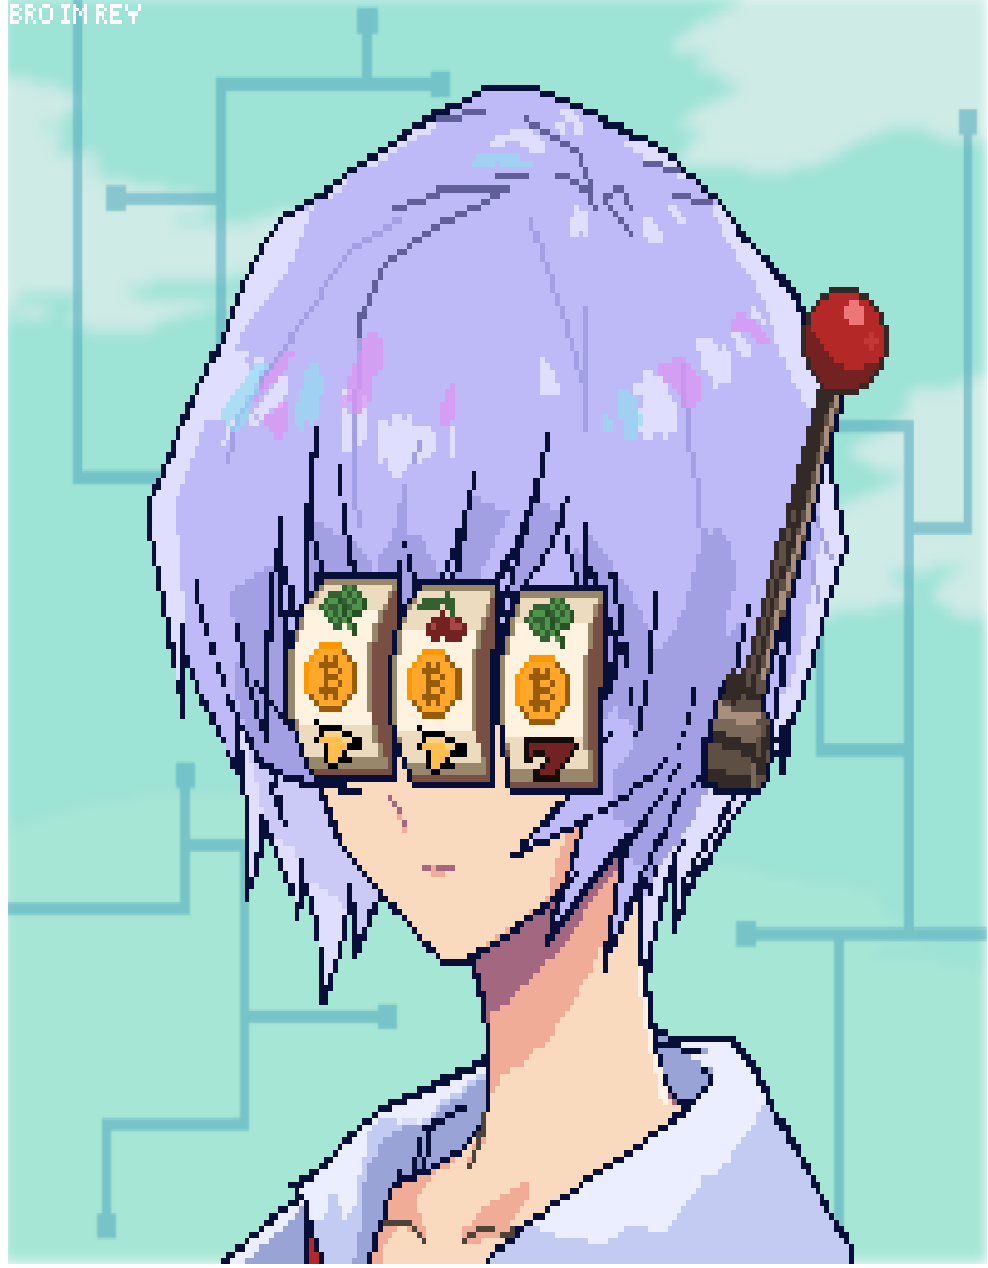
\includegraphics[
        width=\linewidth
    ]{images/example_avatar.png}
\end{minipage}

% ============================================================
% EDUCATION
% ============================================================

\section{
    \texorpdfstring{
    \makebox[\widthof{\faGraduationCap}][c]{
        \color{NA_Red}{\faGraduationCap}
    }\quad Education
    }
    {
    Education
    }
}


\subsection{
    \texorpdfstring{
        MSc in Physics
        \hfill September 2025 -- July 2027
    }{
        MSc in Physics -- September 2025--July 2027
    }
}

\textbf{University of Cair Paravel, Narnia}

\begin{itemize}
    \item Current average grade: 28.4/30.
    \item Relevant subjects: Quantum Mechanics, Computational Physics,
    Statistical Mechanics, and Advanced Mathematical Methods.
    \item Research interests: Particle physics, numerical modeling,
    and scientific computing.
\end{itemize}

\subsection{
    \texorpdfstring{
    BSc in Physics
    \hfill September 2022 -- July 2025
    }
    {BSc in Physics -- September 2022 -- July 2025}
}

\textbf{University of Cair Paravel, Narnia}

\begin{itemize}
    \item Final grade: 110/110.
    \item Bachelor's thesis: Numerical Simulation of Particle Interactions.
    \item Developed Python tools to process simulated data and compare
    numerical results with theoretical predictions.
\end{itemize}

\subsection{
    \texorpdfstring{
    Scientific High School Diploma
    \hfill September 2017 -- June 2022
    }
    {Scientific High School Diploma
    -- September 2017 -- June 2022}
}

\textbf{Experiment House, Cair Paravel}

\begin{itemize}
    \item Final grade: 98/100.
    \item Strong foundation in mathematics, physics, and computer science.
\end{itemize}

% ============================================================
% EXPERIENCE
% ============================================================

\section{
    \texorpdfstring{
    \makebox[\widthof{\faGears}][c]{
        \color{NA_Red}{\faGears}
    }\quad Experience
    }
    {
    Experience
    }
}

\subsection{
    \texorpdfstring{
    Numerical Simulation of Particle Interactions
    \hfill March -- July 2025
    }
    {Numerical Simulation of Particle Interactions
    -- March -- July 2025}
}

\textbf{Undergraduate Research Student}
\hfill University of Cair Paravel

\begin{itemize}
    \item Developed Python scripts to simulate particle interactions
    and investigate numerical models.
    \item Used NumPy and SciPy for numerical calculations and
    Matplotlib for data visualization.
    \item Compared simulation outputs with theoretical predictions
    and investigated numerical errors.
    \item Prepared technical documentation and presented the results
    to an academic supervisor.
\end{itemize}

\subsection{
    \texorpdfstring{
    Computational Physics Winter School
    \hfill February 2026
    }
    {Computational Physics Winter School
    -- February 2026}
}

\textbf{Participant}
\hfill University of Tashbaan 

\begin{itemize}
    \item Attended lectures on numerical methods, quantum mechanics,
    and scientific computing.
    \item Completed practical exercises involving Python-based
    numerical simulations.
    \item Collaborated with students from different academic backgrounds
    on computational physics problems.
\end{itemize}


% ============================================================
% PAGE TWO
% ============================================================

\CVNewPage


\subsection{
    \texorpdfstring{
    University Physics Society
    \hfill September 2024 -- Present
    }
    {
    University Physics Society
    -- September 2024 -- Present
    }
}

\textbf{President}
\hfill University of Cair Paravel

\begin{itemize}
    \item Coordinate a student committee responsible for academic
    and science communication events.
    \item Organize seminars and discussions with researchers
    and university lecturers.
    \item Manage event planning, communications, and collaboration
    with university departments.
\end{itemize}

\subsection{
    \texorpdfstring{
    Science Outreach Programme
    \hfill October 2022 -- Present
    }
    {Science Outreach Programme
    -- October 2022 -- Present}
}

\textbf{Volunteer}
\hfill Cair Paravel, Narnia

\begin{itemize}
    \item Support interactive physics demonstrations for secondary-school
    students.
    \item Explain scientific concepts through experiments and practical
    activities.
    \item Contribute to public engagement initiatives promoting
    STEM education.
\end{itemize}


% ============================================================
% INTERNATIONAL EXPERIENCE
% ============================================================

\section{
    \texorpdfstring{
    \makebox[\widthof{\faGlobe}][c]{
        \color{NA_Red}{\faGlobe}
    }\quad International Experience
    }
    {
    International Experience
    }
}

\subsection{
    \texorpdfstring{
    European Summer School in Particle Physics
    \hfill May 2026
    }
    {European Summer School in Particle Physics
    -- May 2026}
}

\textbf{Visiting Student}
\hfill CERN, Switzerland

\begin{itemize}
    \item Attended introductory seminars on particle detectors,
    accelerator physics, and experimental data analysis.
    \item Explored the role of computational methods in modern
    high-energy physics.
    \item Participated in group discussions on current challenges
    in experimental and theoretical physics.
\end{itemize}

\subsection{
    \texorpdfstring{
    Open Science and Research Software Workshop
    \hfill October 2026
    }
    {
    Open Science and Research Software Workshop
    -- October 2026
    }
}

\textbf{Participant}
\hfill Azim Balda, Calormen

\begin{itemize}
    \item Explored reproducible research workflows and collaborative
    software development.
    \item Practiced version control using Git and GitHub.
    \item Discussed open-source tools and good practices for
    scientific research.
\end{itemize}

% ============================================================
% COMPETITIONS AND AWARDS
% ============================================================

\section{
    \texorpdfstring{
    \makebox[\widthof{\faTrophy}][c]{
        \color{NA_Red}{\faTrophy}
    }\quad Competitions and Awards
    }
    {
    Competitions and Awards
    }
}

\subsection{
    \texorpdfstring{
    National Physics Competition
    \hfill March 2024
    }
    {National Physics Competition
    -- March 2024}
}

\textbf{Individual Competitor}

\begin{itemize}
    \item Reached the national final after qualifying through
    the regional selection.
    \item Demonstrated problem-solving skills in mechanics,
    electromagnetism, and mathematical physics.
\end{itemize}

\subsection{
    \texorpdfstring{
    University Data Analysis Challenge
    \hfill November 2025
    }
    {University Data Analysis Challenge
    -- November 2025}
}

\textbf{Team Member -- Second Place}

\begin{itemize}
    \item Collaborated with two students to analyze a scientific dataset.
    \item Developed Python scripts for data processing and visualization.
    \item Presented the team's methodology and conclusions to a panel
    of evaluators.
\end{itemize}


% ============================================================
% PAGE THREE
% ============================================================

\CVNewPage

% ============================================================
% TECHNICAL SKILLS
% ============================================================

\section{
    \texorpdfstring{%
    \makebox[\widthof{\faWrench}][c]{
        \color{NA_Red}{\faWrench}
    }\quad Technical Skills
    }
    {
    Technical Skills
    }
}

\begin{itemize}
    \item \textbf{Programming:} Python, C++, basic Bash scripting.
    \item \textbf{Scientific computing:} NumPy, SciPy, Matplotlib,
    Jupyter Notebook, ROOT, and PyROOT.
    \item \textbf{Data analysis:} Statistical analysis, numerical modeling,
    data visualization, and uncertainty estimation.
    \item \textbf{Development tools:} Git, GitHub, VS Code, Linux,
    and \LaTeX.
    \item \textbf{Research:} Literature review, technical writing,
    scientific reporting, and reproducible computational workflows.
    \item \textbf{Soft skills:} Teamwork, public speaking,
    problem-solving, and project coordination.
\end{itemize}




% ============================================================
% LANGUAGES
% ============================================================

\section{
    \texorpdfstring{
    \makebox[\widthof{\faLanguage}][c]{
        \color{NA_Red}{\faLanguage}
    }\quad Languages
    }{
    Languages
    }
}

\begin{multicols}{2}
    \begin{itemize}
        \item Narnian : Native
        \item English: C1
        \item German: B1
        \item French: A2
    \end{itemize}
\end{multicols}

% ============================================================
% ADDITIONAL INFORMATION
% ============================================================

\section{
    \texorpdfstring{
        \makebox[\widthof{\faInfo}][c]{
            \color{NA_Red}{\faInfo}
        }\quad Additional Information
    }{
        Additional Information
    }
}

\begin{itemize}
    \item \textbf{Research interests:} Particle physics, computational
    physics, numerical simulations, and scientific software.
    \item \textbf{Interests:} Hiking, chess, science communication,
    and open-source projects.
    \item \textbf{Email:}
    \href{mailto:rei.red@example.com}{rei.red@example.com}
    \item \textbf{GitHub:}
    \href{https://github.com/reired-demo}{github.com/reired-demo}
\end{itemize}

\end{document}